%%
%% This is file `sample-sigconf.tex',
%% generated with the docstrip utility.
%%
%% The original source files were:
%%
%% samples.dtx  (with options: `sigconf')
%% 
%% IMPORTANT NOTICE:
%% 
%% For the copyright see the source file.
%% 
%% Any modified versions of this file must be renamed
%% with new filenames distinct from sample-sigconf.tex.
%% 
%% For distribution of the original source see the terms
%% for copying and modification in the file samples.dtx.
%% 
%% This generated file may be distributed as long as the
%% original source files, as listed above, are part of the
%% same distribution. (The sources need not necessarily be
%% in the same archive or directory.)
%%
%%
%% Commands for TeXCount
%TC:macro \cite [option:text,text]
%TC:macro \citep [option:text,text]
%TC:macro \citet [option:text,text]
%TC:envir table 0 1
%TC:envir table* 0 1
%TC:envir tabular [ignore] word
%TC:envir displaymath 0 word
%TC:envir math 0 word
%TC:envir comment 0 0
%%
%%
%% The first command in your LaTeX source must be the \documentclass command.
\documentclass[sigconf]{acmart}

%%
%% \BibTeX command to typeset BibTeX logo in the docs
\AtBeginDocument{%
  \providecommand\BibTeX{{%
    Bib\TeX}}}

%% Rights management information.  This information is sent to you
%% when you complete the rights form.  These commands have SAMPLE
%% values in them; it is your responsibility as an author to replace
%% the commands and values with those provided to you when you
%% complete the rights form.
\setcopyright{acmcopyright}
\copyrightyear{2023}
\acmYear{2023}
\acmDOI{XXXXXXX.XXXXXXX}

%% These commands are for a PROCEEDINGS abstract or paper.
\acmConference[ICCDA '23]{}{July, 2023}{GuiYang, CN}
\acmPrice{15.00}
\acmISBN{978-1-4503-XXXX-X/23/07}

%%
%% Submission ID.
%% Use this when submitting an article to a sponsored event. You'll
%% receive a unique submission ID from the organizers
%% of the event, and this ID should be used as the parameter to this command.
%%\acmSubmissionID{123-A56-BU3}

%%
%% For managing citations, it is recommended to use bibliography
%% files in BibTeX format.
%%
%% You can then either use BibTeX with the ACM-Reference-Format style,
%% or BibLaTeX with the acmnumeric or acmauthoryear sytles, that include
%% support for advanced citation of software artefact from the
%% biblatex-software package, also separately available on CTAN.
%%
%% Look at the sample-*-biblatex.tex files for templates showcasing
%% the biblatex styles.
%%

%%
%% The majority of ACM publications use numbered citations and
%% references.  The command \citestyle{authoryear} switches to the
%% "author year" style.
%%
%% If you are preparing content for an event
%% sponsored by ACM SIGGRAPH, you must use the "author year" style of
%% citations and references.
%% Uncommenting
%% the next command will enable that style.
%%\citestyle{acmauthoryear}

%%
%% end of the preamble, start of the body of the document source.
\begin{document}

%%
%% The "title" command has an optional parameter,
%% allowing the author to define a "short title" to be used in page headers.
\title{Projit: An Open Source tool for Decoupled Data Science}

%%
%% The "author" command and its associated commands are used to define
%% the authors and their affiliations.
%% Of note is the shared affiliation of the first two authors, and the
%% "authornote" and "authornotemark" commands
%% used to denote shared contribution to the research.
\author{John Hawkins}
\email{john.hawkins@Getting-Data-Science-Done.com}
\orcid{1234-5678-9012}
\affiliation{%
  \institution{Getting-Data-Science-Done.com}
  \city{Sydney}
  \state{NSW}
  \country{Australia}
  \postcode{2000}
}

\renewcommand{\shortauthors}{Hawkins}

\begin{abstract} 
Scientific practice has expanded to become increasingly dependent of digitial technologies,
large scale data processing and advanced analytical methods. These shifts have demanded new
methods of implementing and recording the details of scientific projects. Monolothic applications
have the advantage of a single and consistent design, however they impede the ability of users to
innovate and incrementally improve processes. We discuss the qualities of an ideal eScience framework
for building multi-stage collaboration scinetific workflows and present an open source implementation
for managing scientific processes in a decoupled fashion that permits both flexible implementation of
any stage of processing, and greater ease of meta-data analysis.
\end{abstract}


\keywords{Data Science, Experiment Tracking, Reproducible Science, Metadata Tracking}

\maketitle

\section{Introduction}

Progress in scientific research depends heavily on accurate record keeping of previous
experimental approaches and results. Failure to maintain these records impedes progress
by making it difficult to reproduce work, or imposing the costs of repeatedly testing 
failed lines of experimentation. This cost becomes particularly high in the age of the
reproducibility crisis, as a many teams running the same experiments in parallel, without
knowledge of each others work, has produced a factory line of un-reproducible results.
 
Many Machine Learning experimentation frameworks focus on the task of making experiments
easier to execute and deploy into production systems\cite{Alberti:2018,MolnerDomenech:2020}. 
To do so they are often constructed for specific combinations of technology. This is a necessary limitation 
to enable efficiency, but has the effect of limiting general applicability.
Many other eScience frameworks focus on the lineage and management of data, referred to as 
the so-called provenance problem \cite{Sahoo:2008,Conquest:2021}
The goal of the provenance frameworks is sufficient auditibiliy of data sources that will 
render eScience transparent and repeatable.

Other frameworks and approaches focus on understanding how to do large scale collaborative science, or
facilitate meta-level learning of various kinds\cite{Hunter:2005,Liu:2023}. The better we track the
process of science as a whole, the better we can understand both how to improve scientific processes
as well as data mine the history of science for phenomena that were difficult to detect.

\section{Methodology}

We begin by discussing all desirable elements required of an open science framework. These are drawn
from observations of both how collaborative science works and the successful components of distributed
scientific endeavours. These requirements are drawn from both sciences that are typically dependent
on computational frameworks (computer science, bioinformatics, physics) and those that generally are not
(social science, psychology).

The key elements are as follows:

\begin{itemize}
 \item Sources: Provenance of Data Sources
 \item Processing: Record of Data Processing
 \item Reuse: Facilitating Reuse of Datasets
 \item Tracking: Tracking of Experiments and outputs
 \item Results: Comparison of Methods and Results
 \item Documentation: Generation of Documentation
 \item Reproduction: Reproducibility of Projects
 \item Meta-Analysis: Facilitation of Meta-Analysis
\end{itemize}

The elements in this list are organised in an approximately sequential manner. However, as we discuss
them below it should be apparent that there are many ways in which these elements support each other.
Firstly, and foremost, aata driven projects
require a method of accessing the required \textbf{source} data and will need to maintain records 
of this data provenance. There will typically be \textbf{processing} applied to these datasets to 
render them applicable to experimentation and analysis. An ideal tool will track the sequential 
nature of this processing as well as store information about the location of each resulting dataset.
The data processed in this way is then available for \textbf{reuse} across experiments and analysis,
making \textbf{results} comparable and facilitating \textbf{meta-analysis}. 



\subsection{Projit Process}

The central design principle of \textit{projit} is that the decoupling of data science 
should be achieved through utilisation of a simple metadata store. Each aspect of 
data science work can be allowed to proceed without awareness of the structure of 
any other element as long as it can access the information it requires through this
metadata store.

\begin{figure*}
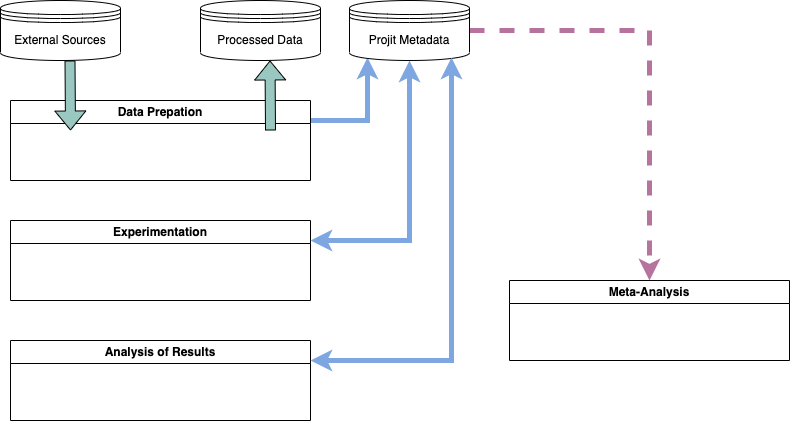
\includegraphics[scale=0.6]{./Projit_decoupled_process.drawio.png}
\caption{Projit Process for Decoupled Data Science}
\label{fig:projit}
\end{figure*}

In Figure \ref{fig:projit} we see that the core steps of data preparation, experimentation
and analysis of results all happen independently. Each of them accesses the projit store for
the information they need, storing information 

\subsection{Application}



\section{Results}



\section{Conclusion}


\section{Acknowledgments}

\bibliographystyle{ACM-Reference-Format}
\bibliography{refs}

\end{document}
\endinput
